\section{Dataset and Released Artifacts}
\label{sec:resource}
\subsection{An inferred resource for process analysis}
The resource is available at \url{https://github.com/fit-alessandro-berti/annotated-egocentric-10k-dataset}. It links generated transcripts, worker summaries, factory vocabularies, inferred events, logs, and analysis artifacts from six factories. Researchers can inspect how events are constructed, compare alternative representations, and examine how activity and process labels affect measurements.

Assembly101~\cite{sener2022assembly101} provides toy assembly and disassembly recordings from static and egocentric cameras, with action annotations for recognition, anticipation, and segmentation. The present resource focuses on the construction of inferred events and their use in process analysis.

The labels and boundaries are inferred by the pipeline. Assessment includes structural checks and an author audit against generated transcripts, without independent video annotations. Comparisons therefore evaluate representation choices unless checked against video; the resource is not a ground-truth benchmark for action recognition or boundary detection.

% Declare the inventory early so it fits at the bottom of page 13.
\begin{table*}[!b]\begin{adjustwidth}{-\extralength}{0cm}
\caption{Artifact inventory. Counts come from the frozen repository outputs. Worker and factory merged logs repeat the same source events.}
\label{tab:inventory}\small
\begin{tabularx}{\linewidth}{@{}l r L@{}}\toprule
Layer & Files & Content and provenance \\\midrule
Generated transcripts & 322 & One text per video; recording identity in path \\
Worker summaries & 59 & One text per worker; combines generated transcripts \\
Factory reports & 6 & Narrative, worker entries, activity and process lists \\
Per-video logs & 322 & 10{,}698 interval-event rows; six stored columns \\
Merged worker logs & 59 & Same 10{,}698 events with source file, worker case, and local offsets \\
Merged factory logs & 6 & Same 10{,}698 events concatenated across workers \\
Audit record & 1 & 42 event-support judgments and 42 transcript-entry-overlap judgments \\
Prompts; stage scripts & 4; 5 & Extraction instructions and implementation \\
\bottomrule\end{tabularx}
\end{adjustwidth}\end{table*}

\subsection{Selection and provenance}
The archived subset contains outputs for factories \textbf{001} to \textbf{006}, with 59 worker identifiers and 322 paired generated transcript and event files. Factory and worker identifiers are inherited from the source organization. Domain descriptions in this paper summarize generated factory reports; they are not independently verified factory metadata. The archive does not record the selection rationale, the original source revision, or a complete inventory of the recordings available at extraction time. We therefore describe an available processed subset, not a random or representative sample of factories.

The current provider card reports a median clip length of 180 seconds~\cite{build2025egocentric}, whereas many archived generated transcript endpoints lie near 20 minutes. These describe different quantities and possibly different snapshots or subsets. The card documents a per-video \texttt{duration\_sec} field inside source archives, but those metadata files are not included here. The pipeline scans video files and does not preserve that field. The selected recordings' actual durations therefore cannot be established from the derived archive. The inspected public dataset snapshot does not identify the historical source version used for extraction.

The six per-video columns are \texttt{start\_timestamp}, \texttt{end\_timestamp}, \texttt{activity}, \texttt{process}, \texttt{factory}, and \texttt{worker}. \textbf{S5} adds \texttt{source\_file}, \texttt{case\_id}, video-relative start and end offsets, and duration. Table~\ref{tab:inventory} distinguishes file counts from unique event counts. The released dataset documentation follows the documentation concerns of Datasheets for Datasets~\cite{gebru2021datasheets}: composition, collection, uses, and limitations.

There are 13{,}304 generated transcript entries recognized by the original three-component timestamp parser. Recognizing the additional two-component and mixed-format entries gives 13{,}462 entries, without rescaling any timestamp.

Across all logs, the original endpoint-span calculation totals 786{,}412 seconds (218.4 hours). This sums parsed spans, not verified footage durations. Interval unions cover 414{,}886 seconds by counting overlapping time only once. Summed event durations total 421{,}283 seconds because each row contributes its full duration. Their difference, 6{,}397 seconds, is the additional time counted through overlaps.

The retained time-analysis subset contains 10{,}647 events in 320 logs, with 349{,}659 seconds of summed event duration (97.1 hours). This is the duration used for category shares; it is neither the full archive's endpoint span nor its interval-union duration.

\subsection{Timestamp formats and inclusion rules}
\label{sec:temporal}
The time analysis excludes a log if any event ends more than one hour after the start of its recording. This rule uses event times, so an unusual timestamp in a generated transcript does not automatically exclude its log. It removes two logs, both from factory \textbf{001}, and keeps the other five in Table~\ref{tab:anomalies}. Keeping a log does not confirm that its timestamps are correct.

\begin{table*}[!b]\begin{adjustwidth}{-\extralength}{0cm}
\caption{Latest end times in seven generated transcripts and their event logs. All times are shown as hours:minutes:seconds. The transcript times exceed one hour, but a log is excluded from the time analysis only if an event end time exceeds one hour. IDs indicate factory/worker/video. Actual video durations are unknown.}
\label{tab:anomalies}\small
\begin{tabular}{@{}llll@{}}\toprule
ID & Generated transcript endpoint & Event endpoint & Time-analysis decision \\\midrule
\textbf{001}/001/00004 & 20:00:00 & 20:00:00 & Exclude \\
\textbf{001}/010/00001 & 01:20:00 & 01:20:00 & Exclude \\
\textbf{002}/002/00008 & 20:00:00 & 00:20:00 & Retain \\
\textbf{002}/010/00001 & 20:00:00 & 00:20:00 & Retain \\
\textbf{005}/002/00000 & 13:52:00 & 00:13:52 & Retain \\
\textbf{006}/001/00001 & 20:06:00 & 00:20:06 & Retain \\
\textbf{006}/004/00000 & 19:59:00 & 00:19:59 & Retain \\
\bottomrule\end{tabular}
\end{adjustwidth}\end{table*}

Table~\ref{tab:anomalies} compares the latest end times in the seven generated transcripts that exceed one hour when read as hours:minutes:seconds. For example, one transcript ends at \texttt{20:06:00}, while its event log ends at \texttt{00:20:06}. This may reflect a timestamp-format error, but the available data do not establish which time is correct. We keep the recorded timestamps without correcting or rescaling them.

Timestamp formats also affect how many transcript entries can be read. The original parser accepts only \texttt{HH:MM:SS} (hours:minutes:seconds). An additional check also accepts \texttt{MM:SS} (minutes:seconds) and files that mix both formats. Four other transcripts contain \texttt{MM:SS} times: \textbf{001}/004/00001, \textbf{002}/005/00001, \textbf{002}/009/00003, and \textbf{003}/003/00003. Three mix formats; \textbf{002}/005/00001 uses \texttt{MM:SS} throughout. The original parser misses 158 entries in these files, explaining the different entry counts reported above.

These timestamp inconsistencies affect the coverage ratios in Section~\ref{sec:consistency}. A low ratio alone does not show that extraction missed later parts of a long video.

\subsection{Synthetic time and case selection}
\label{sec:cases}
Each recording has its own local timeline. To combine recordings into a worker sequence, the merge shifts their event times onto a common artificial timeline. \textbf{S4} stores local offsets as dates relative to 2000-01-01 for software compatibility. The archive provides no verified calendar times or cross-worker synchronization. \textbf{S5} processes clips in filename order, which is not proof of their real chronological order.

For a worker's ordered clips $v_1,\ldots,v_m$, the last extracted event endpoint in recording $j$ is $M_j=\max_{e\in E_{v_j}}t_e$, with $M_j=0$ for an empty log. Let $O_j$ be the accumulated time shift for that recording, and let the primed endpoints be the shifted event times. \textbf{S5} adds the preceding recording's endpoint to the accumulated shift and applies it to each event:
\begin{equation}
 O_1=0,\qquad O_{j+1}=O_j+M_j,\qquad
 (t_s',t_e')=(O_j+t_s,O_j+t_e).
\end{equation}
The same shift is added to both endpoints, preserving the event's duration. For example, if the first recording's last extracted endpoint is 60 seconds, an event at 10 to 20 seconds in the next recording appears at 70 to 80 seconds. The next clip starts at the largest extracted endpoint, not at the full source duration. Unrepresented trailing footage and empty logs add no elapsed time. Within-clip gaps before that endpoint remain on the synthetic axis, but gaps between recording sessions are unknown. Each worker has a separate synthetic origin; equal synthetic dates do not establish simultaneous work.

\begin{figure*}[!t]\begin{adjustwidth}{-\extralength}{0cm}\centering
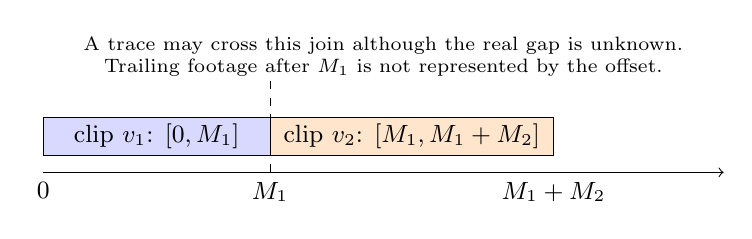
\begin{tikzpicture}[x=0.72cm,y=0.7cm,font=\small]
\draw[->] (0,0)--(12,0);
\draw[fill=blue!15] (0,0.3) rectangle (4,1);
\draw[fill=orange!20] (4,0.3) rectangle (9,1);
\node at (2,0.65){clip $v_1$: $[0,M_1]$};
\node at (6.5,0.65){clip $v_2$: $[M_1,M_1+M_2]$};
\node[below] at (0,0){0};\node[below] at (4,0){$M_1$};\node[below] at (9,0){$M_1+M_2$};
\draw[dashed] (4,0)--(4,1.7);
\node[align=center,font=\scriptsize] at (6,2.1){A trace may cross this join although the real gap is unknown.\\Trailing footage after $M_1$ is not represented by the offset.};
\end{tikzpicture}
\caption{Schematic of the implemented merge, not measured source time. The first clip occupies the synthetic span from zero to its last extracted endpoint; the second starts there and adds its own endpoint span. Separate video cases preserve the clip boundary. A worker case creates a directly-follows relation across it.}
\label{fig:synthetic}\end{adjustwidth}\end{figure*}

\begin{table*}[!b]\begin{adjustwidth}{-\extralength}{0cm}
\caption{Case constructions supported by the attributes. Process episodes require an additional grouping step and are not stored as case IDs.}
\label{tab:cases}\footnotesize
\begin{tabularx}{\linewidth}{@{}p{0.22\linewidth}LL@{}}\toprule
Case rule & Supported description & Interpretation risk \\\midrule
Video as case, $\kappa(e)=v$ & Local activity order within an observation window; used for discovery & Window may start or end midway through a production process \\
Worker as case, $\kappa(e)=(f,w)$ & Sequence of retained clips; stored \textbf{S5} case ID & Filename joins can create artificial transitions; calendar duration is unknown \\
Contiguous process episode & Consecutive events with the same process within a chosen clip, with a stated gap rule & Inferred context boundaries do not identify items or completed instances \\
\bottomrule\end{tabularx}
\end{adjustwidth}\end{table*}
\noindent Figure~\ref{fig:synthetic} illustrates the synthetic clip join, and Table~\ref{tab:cases} compares the case rules supported by the released attributes.
